\begin{titlepage}
 \begin{center}
 \newcommand{\HRule}{\rule{\linewidth}{0.5mm}}
% Upper part of the page. The '~' is needed because \\
% only works if a paragraph has started.

\textsc{\LARGE Portland State University}\\[1.5cm]

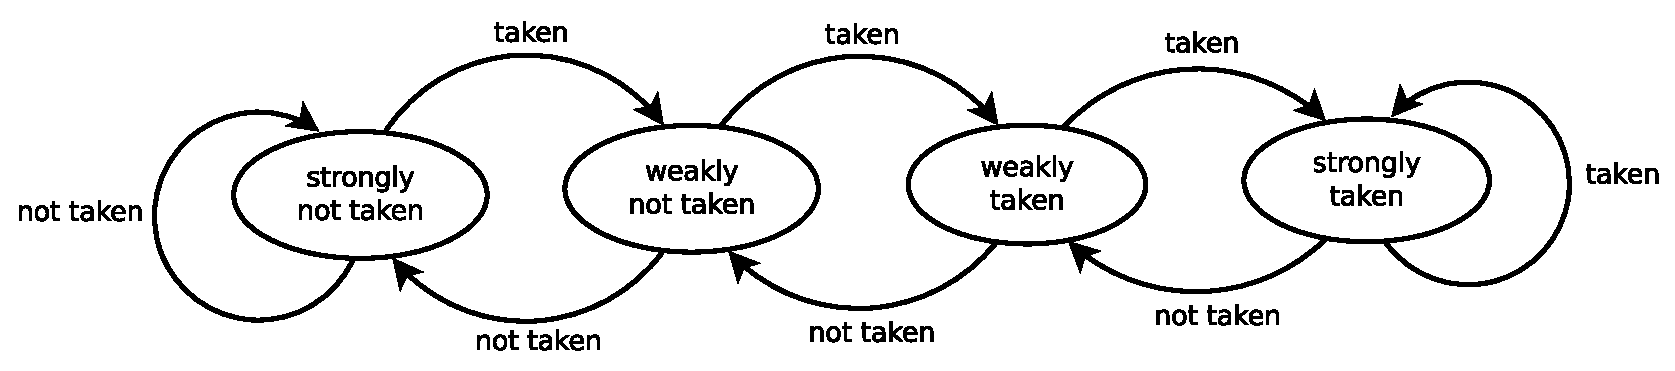
\includegraphics[width=0.5\textwidth]{../latex_common/logo}~\\[1cm]

\textsc{\Large \SUBJECT}\\[0.5cm]

% Title
\HRule \\[0.4cm]
{ \huge \bfseries \TOPIC}\\[0.4cm]

\HRule \\[1.5cm]

% Author and supervisor
\begin{minipage}{0.4\textwidth}
\begin{flushleft} \large
\emph{Author:}\\
\AUTHOR
\end{flushleft}
\end{minipage}
\begin{minipage}{0.4\textwidth}
\begin{flushright} \large
\emph{Instructor:} \\
\INSTRUCTOR
\end{flushright}
\end{minipage}

\vfill

% Bottom of the page
{\large \today}

\end{center}

\end{titlepage}
